\documentclass[a4paper,table]{report}
\input{preamble.tex}
\newcommand{\vect}[2]{(#1_1,\ldots, #1_#2)}
%%%%%%% nesting newcommands $$$$$$$$$$$$$$$$$$$
\newcommand{\function}[1]{\newcommand{\nvec}[2]{#1(##1_1,\ldots, ##1_##2)}}

\newcommand{\linode}[2]{#1_n(x)#2^{(n)}+#1_{n-1}(x)#2^{(n-1)}+\cdots +#1_0(x)#2=g(x)}

\newcommand{\vecoffun}[3]{#1_0(#2),\ldots ,#1_#3(#2)}

\newcommand{\suma}{\sum_{n=0}^{\infty}a_n x^n}

\newcommand{\sumb}{\sum_{n=1}^{\infty}a_n n x^{n-1}}

\newcommand{\sumc}{\sum_{n=2}^{\infty}a_n n (n-1) x^{n-2}}

\newcommand{\varsum}[2]{\sum_{n=#1}^{#2}}
\input{tikz.tex}
\input{myboxes.tex}

\usepackage[cmtip,all]{xy}
\usepackage{silence}
\WarningsOff[catoptions]
\usepackage{extarrows}

\geometry{left=9mm,right=9mm,top=30.00mm,bottom=34.00mm,footskip=24.16mm,headsep=24.16mm}
\everymath{\displaystyle}
\pagestyle{vangelis}

\begin{document}


\chapter{Παράγωγος Σύνθετων Συναρτήσεων}

\section{1η Περίπτωση: \ensuremath{z=f(x,y),  x=x(t),  y=y(t)}} 

\begin{thm}
  Αν η συνάρτηση $ f(x,y) $ είναι ορισμένη στο ανοιχτό σύνολο 
  $ A \subseteq \mathbb{R}^{2} $ και $ x = x(t) $, $ y=y(t) $, με 
  $ t \in [a,b] $ και η $f$ έχει συνεχείς μερικές 
  παραγώγους στο $A$ και οι $ x(t) $ και $ y(t) $ είναι παραγωγίσιμες στο 
  $ [a,b] $, τότε η παράγωγος της σύνθετης συνάρτησης $f$ ως προς $t$ δίνεται από 
  τον τύπο:

  \vspace{\baselineskip}

  \twocolumnsideslc{
    \begin{center}
      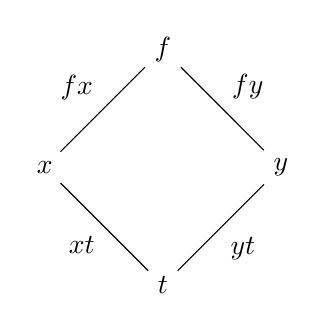
\begin{tikzpicture}
        \node (f) at (0,0) {$f$};  
        \node (x) at (-1.5,-1.5) {$x$};  
        \node (y) at (1.5,-1.5) {$y$};  
        \node (t) at (0,-3) {$t$};  
        \draw (f) edge node[midway,above left] {$\pdv{f}{x}$} (x) ;
        \draw (f) edge node[midway,above right] {$\pdv{f}{y}$} (y) ;
        \draw (x) edge node[midway,below left] {$\dv{x}{t}$} (t) ;
        \draw (y) edge node[midway,below right] {$\dv{y}{t}$} (t) ;
      \end{tikzpicture}
    \end{center}
  }{
    \begin{equation}\label{eq:deriv1}
      \dv{f}{t} = \pdv{f}{x} \dv{x}{t} + \pdv{f}{y} \dv{y}{t} 
    \end{equation}
    Ενώ η 2η παράγωγος από τον τύπο:
    \[
      \dv[2]{f}{t} =  \pdv[2]{f}{x} \left(\dv{x}{t}\right)^{2} + 
      2 \pdv[2]{f}{x}{y} \dv{x}{t} \dv{y}{t} + \pdv[2]{f}{y} 
      \left(\dv{y}{t}\right)^{2} + \pdv{f}{x} \dv[2]{x}{t} + \pdv{f}{y} \dv[2]{y}{t}
    \]
  }
\end{thm}

\section{2η Περίπτωση: \ensuremath{z=f(x,y),  x=x(u,v),  y=y(u,v)}} 

\begin{thm}
  Αν η συνάρτηση $ f(x,y) $ είναι ορισμένη στο ανοιχτό σύνολο 
  $ A \subseteq \mathbb{R}^{2} $ και $ x = x(u,v) $, $ y=y(u,v) $, με 
  και η $f$ έχει συνεχείς μερικές παραγώγους στο $A$ και οι $ x $ και $ y $, έχουν 
  συνεχείς μερικές παραγώγους στο $ E \subseteq \mathbb{R}^{2} $,
  τότε οι μερικές παράγωγοι της $f$, υπάρχουν και δίνονται από τους τύπους:
\end{thm}

\twocolumnsideslc{ 
  \begin{center}
    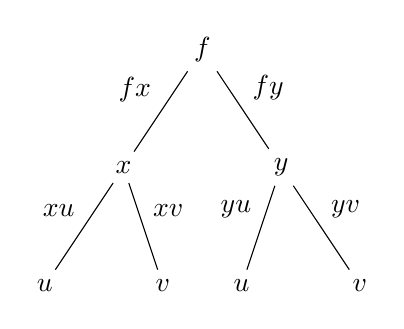
\begin{tikzpicture}
      \node (f) at (0,0) {$f$};  
      \node (x) at (-1,-1.5) {$x$};  
      \node (y) at (1,-1.5) {$y$};  
      \node (ux) at (-2,-3) {$u$};  
      \node (vx) at (-0.5,-3) {$v$};  
      \node (uy) at (0.5,-3) {$u$};  
      \node (vy) at (2,-3) {$v$};  
      \draw (f) edge node[midway,above left] {$ \pdv{f}{x}$} (x) ;
      \draw (f) edge node[midway,above right] {$ \pdv{f}{y}$} (y) ;
      \draw (x) edge node[midway,above left] {$ \pdv{x}{u}$} (ux) ;
      \draw (x) edge node[midway,above right] {$ \pdv{x}{v}$} (vx) ;
      \draw (y) edge node[midway,above left] {$ \pdv{y}{u}$} (uy) ;
      \draw (y) edge node[midway,above right] {$ \pdv{y}{v}$} (vy) ;
    \end{tikzpicture}  
  \end{center}
}{
  \begin{equation}
    \label{eq:deriv2}
    \pdv{f}{u} = \pdv{f}{x} \pdv{x}{u} + \pdv{f}{y} \pdv{y}{u} 
    \quad \text{και} \quad
    \pdv{f}{v} = \pdv{f}{x} \pdv{x}{v} + \pdv{f}{y} \pdv{y}{v} 
  \end{equation}
  Ενώ οι μερικές παράγωγοι 2ης τάξης, δίνονται από τους τύπους:
  \[
    \pdv[2]{f}{u} =  \pdv[2]{f}{x} \left(\pdv{x}{u}\right)^{2} + 
    2 \pdv[2]{f}{x}{y} \pdv{x}{u} \pdv{y}{u} + \pdv[2]{f}{y} 
    \left(\pdv{y}{u}\right)^{2} + \pdv{f}{x} \pdv[2]{x}{u} + \pdv{f}{y} 
    \pdv[2]{y}{u}
  \]
  \[
    \pdv[2]{f}{v} =  \pdv[2]{f}{x} \left(\pdv{x}{v}\right)^{2} + 
    2 \pdv[2]{f}{x}{y} \pdv{x}{u} \pdv{y}{v} + \pdv[2]{f}{y} 
    \left(\pdv{y}{v}\right)^{2} + \pdv{f}{x} \pdv[2]{x}{v} + \pdv{f}{y} 
    \pdv[2]{y}{v}
  \]
  \[
    \pdv[2]{f}{v}{u} = \pdv[2]{f}{x} \pdv{x}{u} \pdv{x}{v} + \pdv[2]{f}{x}{y}
    \left(\pdv{x}{u} \pdv{y}{v}+ \pdv{x}{v} \pdv{y}{u} \right) + \pdv[2]{f}{y} 
    \pdv{y} {u} \pdv{y}{v} + \pdv{f}{x} \pdv[2]{x}{u}{v} + \pdv{f}{y} 
    \pdv[2]{y}{u}{v} 
  \]
}


\enlargethispage{\baselineskip}

\begin{rem}
  Οι τύποι~\eqref{eq:deriv1} και~\eqref{eq:deriv2} προέκυψαν αθροίζοντας κάθε φορά, 
  τα μονοπάτια που ξεκινούν από τη μεταβλητή $f$ και καταλήγουν στη μεταβλητή ως 
  προς την οποία παραγωγίζουμε, όπου κάθε μονοπάτι αποτελείται από το γινόμενο των 
  παραγώγων που συναντούμε "διασχίζοντάς" το.
\end{rem}


\section{Αποδείξεις των τύπων των μερικών Παραγώγων 2ης τάξης}

\subsection{Απόδειξη με το συμβολισμό του Leibnitz}

Αποδεικνύουμε τον τύπο για την $ \pdv[2]{f}{u} $ και ομοίως προκύπτουν και οι τύποι 
για τις $ \pdv[2]{f}{v}  $ και $ \pdv[2]{f}{u}{v} $.

\vspace{\baselineskip}

\twocolumnsideslc
{
  \begin{center}
    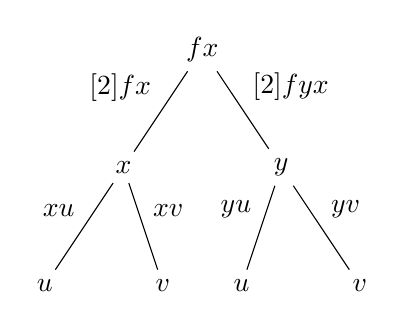
\begin{tikzpicture}
      \node (f) at (0,0) {$ \pdv{f}{x} $};  
      \node (x) at (-1,-1.5) {$x$};  
      \node (y) at (1,-1.5) {$y$};  
      \node (ux) at (-2,-3) {$u$};  
      \node (vx) at (-0.5,-3) {$v$};  
      \node (uy) at (0.5,-3) {$u$};  
      \node (vy) at (2,-3) {$v$};  
      \draw (f) edge node[midway,above left] {$ \pdv[2]{f}{x}$} (x) ;
      \draw (f) edge node[midway,above right] {$ \pdv[2]{f}{y}{x}$} (y) ;
      \draw (x) edge node[midway,above left] {$ \pdv{x}{u}$} (ux) ;
      \draw (x) edge node[midway,above right] {$ \pdv{x}{v}$} (vx) ;
      \draw (y) edge node[midway,above left] {$ \pdv{y}{u}$} (uy) ;
      \draw (y) edge node[midway,above right] {$ \pdv{y}{v}$} (vy) ;
    \end{tikzpicture}  
  \end{center}

  \begin{center}
    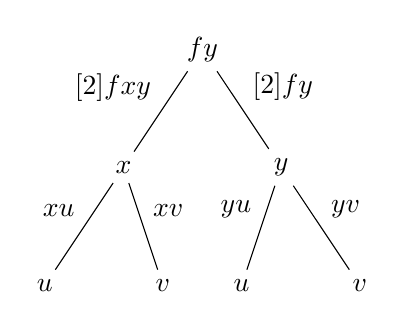
\begin{tikzpicture}
      \node (f) at (0,0) {$ \pdv{f}{y} $};  
      \node (x) at (-1,-1.5) {$x$};  
      \node (y) at (1,-1.5) {$y$};  
      \node (ux) at (-2,-3) {$u$};  
      \node (vx) at (-0.5,-3) {$v$};  
      \node (uy) at (0.5,-3) {$u$};  
      \node (vy) at (2,-3) {$v$};  
      \draw (f) edge node[midway,above left] {$ \pdv[2]{f}{x}{y}$} (x) ;
      \draw (f) edge node[midway,above right] {$ \pdv[2]{f}{y}$} (y) ;
      \draw (x) edge node[midway,above left] {$ \pdv{x}{u}$} (ux) ;
      \draw (x) edge node[midway,above right] {$ \pdv{x}{v}$} (vx) ;
      \draw (y) edge node[midway,above left] {$ \pdv{y}{u}$} (uy) ;
      \draw (y) edge node[midway,above right] {$ \pdv{y}{v}$} (vy) ;
    \end{tikzpicture}  
  \end{center}
}{
  \begin{proof}
    \[
      \begin{aligned}
        \pdv[2]{f}{u} 
  &= \pdv{}{u}\left(\pdv{f}{u}\right) = \pdv{}{u} 
  \left( \pdv{f}{x} \pdv{x}{u} + \pdv{f}{y} \pdv{y}{u}\right) = 
  \pdv{}{u} \left(\pdv{f}{x} \pdv{x}{u}\right) + \pdv{}{u} 
  \left(\pdv{f}{y} \pdv{y}{u}\right) \\
  &= \pdv{}{u} \left( \pdv{f}{x}\right) \pdv{x}{u} + \pdv{f}{x} \pdv{}{u} \left(
  \pdv{x}{u} \right) + \pdv{}{u} \left(\pdv{f}{y} \right) \pdv{y}{u} + \pdv{f}{y} 
  \pdv{}{u} \left(\pdv{y}{u}\right) \\
  &=\left[ \pdv[2]{f}{x} \pdv{x}{u} + \pdv[2]{f}{x}{y} \pdv{y}{u} \right] \pdv{x}{u} +
  \pdv{f}{x} \pdv[2]{x}{u} + 
  \left[ \pdv[2]{f}{y}{x} \pdv{x}{u} + \pdv[2]{f}{y} \pdv{y}{u} \right] \pdv{y}{u} +
  \pdv{f}{y} \pdv[2]{y}{u} \\
  &= \pdv[2]{f}{x} \left(\pdv{x}{u}\right)^{2} + \pdv[2]{f}{x}{y} \pdv{y}{u}
  \pdv{x}{u} + \pdv{f}{x} \pdv[2]{x}{u} + \pdv[2]{f}{y}{x} \pdv{x}{u} \pdv{y}{u} + 
  \pdv[2]{f}{y} \left(\pdv{y}{u}\right)^{2} +
  \pdv{f}{y} \pdv[2]{y}{u} \\
  &= \pdv[2]{f}{x} \left(\pdv{x}{u}\right)^{2} + 2\pdv[2]{f}{x}{y} \pdv{x}{u}
  \pdv{y}{u} + \pdv[2]{f}{y} \left(\pdv{y}{u}\right)^{2} + \pdv{f}{x} \pdv[2]{x}{u} +
  \pdv{f}{y} \pdv[2]{y}{u} \\
      \end{aligned}
    \]
  \end{proof}
}


\subsection{Απόδειξη με το συμβολισμό των δεικτών}

Αποδεικνύουμε τον τύπο για την $ f_{uu} $ και ομοίως προκύπτουν και οι τύποι για τις  
$ f_{vv} $ και $ f_{uv} $.

\vspace{\baselineskip}

\twocolumnsideslc{
\begin{center}
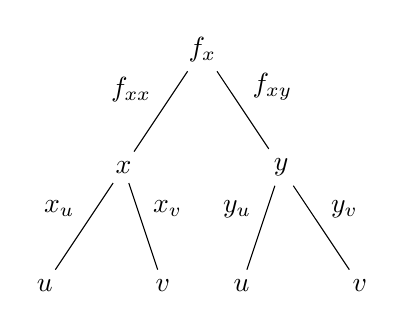
\begin{tikzpicture}
  \node (f) at (0,0) {$f_{x}$};  
  \node (x) at (-1,-1.5) {$x$};  
  \node (y) at (1,-1.5) {$y$};  
  \node (ux) at (-2,-3) {$u$};  
  \node (vx) at (-0.5,-3) {$v$};  
  \node (uy) at (0.5,-3) {$u$};  
  \node (vy) at (2,-3) {$v$};  
  \draw (f) edge node[midway,above left] {$f_{xx}$} (x) ;
  \draw (f) edge node[midway,above right] {$f_{xy}$} (y) ;
  \draw (x) edge node[midway,above left] {$x_{u}$} (ux) ;
  \draw (x) edge node[midway,above right] {$x_{v}$} (vx) ;
  \draw (y) edge node[midway,above left] {$y_{u}$} (uy) ;
  \draw (y) edge node[midway,above right] {$y_{v}$} (vy) ;
\end{tikzpicture}
\end{center}

\begin{center}
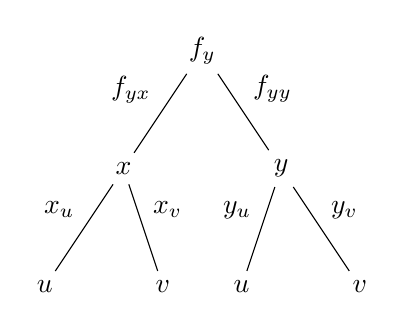
\begin{tikzpicture}
  \node (f) at (0,0) {$f_{y}$};  
  \node (x) at (-1,-1.5) {$x$};  
  \node (y) at (1,-1.5) {$y$};  
  \node (ux) at (-2,-3) {$u$};  
  \node (vx) at (-0.5,-3) {$v$};  
  \node (uy) at (0.5,-3) {$u$};  
  \node (vy) at (2,-3) {$v$};  
  \draw (f) edge node[midway,above left] {$f_{yx}$} (x) ;
  \draw (f) edge node[midway,above right] {$f_{yy}$} (y) ;
  \draw (x) edge node[midway,above left] {$x_{u}$} (ux) ;
  \draw (x) edge node[midway,above right] {$x_{v}$} (vx) ;
  \draw (y) edge node[midway,above left] {$y_{u}$} (uy) ;
  \draw (y) edge node[midway,above right] {$y_{v}$} (vy) ;
\end{tikzpicture}
\end{center}
}{
  \begin{proof}
    \[
      \begin{aligned}
        f_{uu} &= (f_{u})_{u} = (f_{x}x_{u}+f_{y}y_{u})_{u} \\
               &=(f_{x}x_{u})_{u}+ (f_{y}y_{u})_{u} \\
               &=(f_{x})_{u}x_{u} + f_{x}(x_{u})_{u} + (f_{y})_{u}y_{u}+ 
               f_{y}(y_{u})_{u} \\
               &= (f_{xx}x_{u}+f_{xy}{y_{u}})x_{u} + f_{x} x_{uu} + 
               (f_{yx}x_{u}+f_{yy}y_{u})y_{u} + f_{y}y_{uu} \\
               &= f_{xx}(x_{u})^{2} + f_{xy}y_{u}x_{u}+ f_{x}x_{uu} + 
               f_{yx}x_{u}y_{u}+f_{yy}(y_{u})^{2}+ f_{y}y_{uu} \\
               &= f_{xx}(x_{u})^{2}+ 2f_{xy}x_{u}y_{u} + f_{yy}(y_{u})^{2} + 
               f_{x}x_{uu} + f_{y}y_{uu}
      \end{aligned}
    \] 
  \end{proof}
}

\begin{rem}
  Συγκεντρωτικά οι τύποι για τις παραγώγους 2ης τάξης της συνάρτησης 
  \[
    f_{uu}= f_{xx}(x_{u})^{2}+ 2f_{xy}x_{u}y_{u} + f_{yy}(y_{u})^{2} + f_{x}x_{uu} + 
    f_{y}y_{uu} 
  \] 
  \[
    f_{vv}= f_{xx}(x_{v})^{2}+ 2f_{xy}x_{v}y_{v} + f_{yy}(y_{v})^{2} + f_{x}x_{vv} + 
    f_{y}y_{vv} 
  \]
  \[
    f_{uv}= f_{xx}x_{u}x_{v}+ f_{xy}(x_{u}y_{v} + x_{v}y_{u}) + 
    f_{yy}y_{u}y_{v} + f_{x}x_{uv} + f_{y}y_{v} 
    f_{y}y_{vv} 
  \]
\end{rem}



\chapter{Ομογενείς Συναρτήσεις}

\section{Ορισμός}

\begin{dfn}
\item {}
  \begin{enumerate}[i)]
    \item $ f(x,y) $ \textcolor{Col1}{ομογενής βαθμού} $ \textcolor{Col1}{\rho} 
      \Leftrightarrow f(\lambda x, \lambda y), \; \forall \lambda \in \mathbb{R} $ 
    \item $ f(x,y,z) $ \textcolor{Col1}{ομογενής βαθμού} $ \textcolor{Col1}{\rho} 
      \Leftrightarrow f(\lambda x, \lambda y, \lambda z), \; \forall \lambda \in 
      \mathbb{R} $ 
  \end{enumerate}
\end{dfn}

\begin{thm}[Euler]
  Αν $ f(x,y) $ είναι ομογενής βαθμού $ \rho $ τότε $x f_{x} + y f_{y} = \rho f $.
\end{thm}
\begin{prop}
  Αν $ f(x,y) $ είναι ομογενής βαθμού $ \rho $ τότε οι συναρτήσεις 
  $f_{x}, f_{y} $ είναι ομογενείς βαθμού $ \rho -1 $.
\end{prop}
\begin{proof}
\item {}
  $ f $ ομογενής βαθμού $ \rho \overset{\text{(Euler)}}{\Rightarrow} xf_{x}+yf_{y}= 
  \rho f \xRightarrow[\text{ως προς $x$}]{\text{παρ/ζω}} f_{x} + x f_{xx} + y f_{yx} =
  \rho f_{x} \Rightarrow xf_{xx} + yf_{xy} = (\rho -1)f_{x} $

  $ f $ ομογενής βαθμού $ \rho \overset{\text{(Euler)}}{\Rightarrow} xf_{x}+yf_{y}= 
  \rho f \xRightarrow[\text{ως προς $y$}]{\text{παρ/ζω}} xf_{xy} + f_{y} + y f_{yy} =
  \rho f_{y} \Rightarrow xf_{yx} + yf_{yy} = (\rho -1)f_{y} $
\end{proof}

\begin{exercise}
  Έστω $ f(x,y) $, συνεχής, με συνεχείς μερικές παραγώγους 2ης τάξης, 
  ομογενής βαθμού $\rho$. Να δείξετε ότι ισχύει \[ x^{2}f_{xx}+2xyf_{xy}+y^{2}f_{yy} =
  \rho (\rho -1)f \]
\end{exercise}
\begin{solution}
\item {}
  $f$ ομογενής βαθμού $\rho \Rightarrow f_{x}, f_{y} $ ομογενείς βαθμού $\rho -1$.
  Οπότε ισχύει το θεώρημα Euler για αυτές, άρα:
  \begin{align*}
    \sysdelim.\}\systeme{x f_{xx}+yf_{xy}=(\rho -1)f_{x}, x f_{yx}+yf_{yy}=
  (\rho -1)f_{y}} \Rightarrow \sysdelim.\}
  \systeme*{x^{2} f_{xx} \+ xyf_{xy}=(\rho-1)xf_{x},yxf_{yx} \+ y^{2}f_{yy}=
  (\rho -1)yf_{y}} \xRightarrow{(+)} x^{2}f_{xx}+2xyf_{xy}+y^{2}f_{yy}=
  (\rho -1)(xf_{x}+yf_{y})
\end{align*} 
Όμως επειδή $f$ ομογενής έχουμε ότι $ xf_{x}+yf_{y}= \rho f $. Οπότε
\[
  x^{2}f_{xx}+2xyf_{xy}+y^{2}f_{yy} = \rho (\rho -1)f
\] 
\end{solution}


\begin{exercise}
  Αν $ u = u(x,y) $ και $ v=v(x,y) $ ομογενείς βαθμού $ \rho $, 
  τότε να δείξετε ότι $ \forall f(u,v) $ με συνεχείς μερικές παραγώγους 1ης τάξης
  ισχύει 
  \[
    xf_{x}+yf_{y}= \rho (u f_{u}+vf_{v}) 
  \] 
\end{exercise}
\begin{solution}
\item {}
  Έχουμε ότι για τις συναρτήσεις $u(x,y) $ και $v(x,y)$ είναι ομογενείς 
  βαθμού $\rho$, οπότε:
  \[
  \sysdelim.\}\systeme{xu_{x}+yu_{y}= \rho u, xv_{x}+yv_{y}= \rho v} 
\] 
Για την συνάρτηση $f$ έχουμε ότι είναι σύνθετη με $ f=f(u,v) $ και 
$ u = u(x,y) $ και $ v=v(x,y) $, οπότε οι μερικές παράγωγοί της δίνονται από
το δέντρο της και είναι:
\[
  \left.
    \begin{tabular}{l}
      $f_{x}=f_{u}u_{x}+f_{v}v_{x}$ \\
      $f_{y}=f_{u}u_{y}+f_{v}v_{y}$
    \end{tabular}
  \right\}
  \Rightarrow xf_{x}+yf_{y} = \underbrace{(xu_{x}+yu_{y})}_{\rho
  u}f_{u}+\underbrace{(xv_{x}+yv_{y})}_{\rho v}f_{v}
\] 
Άρα 
\[
  xf_{x}+yf_{y} = \rho (uf_{u}+vf_{v}) 
\] 
\end{solution}

\begin{exercise}
  Έστω $ u = u(x,y) $ και $ v = v(x,y) $, ομογενείς βαθμού $\rho$, με 
  $ u(x,y) \neq 0, v(x,y) \neq 0, \; \forall (x,y) \in \mathbb{R}^{2} $. 
  Να δείξετε ότι 
  \[
    udv -v du = \frac{1}{\rho} \pdv{(u,v)}{(x,y)} (xdy-ydx) 
    \quad \text{όπου} \quad  \pdv{(u,v)}{(x,y)} = 
    \begin{vmatrix}
      u_{x} & u_{y} \\ v_{x} & v_{y} 
    \end{vmatrix} 
  \] 
\end{exercise}
\begin{solution}
  \[
    \left.
      \begin{matrix}
        du=u_{x}dx+u_{y}dy \\
        dv=v_{x}dx+v_{y}dy
      \end{matrix} 
    \right\} \Rightarrow 
    \left.
      \begin{matrix}
        vdu=vu_{x}dx+vu_{y}dy \\ 
        udv=uv_{x}dx+uv_{y}dy
      \end{matrix} 
    \right\} \overset{(-)}{\Rightarrow} 
    udv -vdu = (uv_{x}-vu_{x})dx+(uv_{y}-vu_{y})dy 
  \] 

  \begin{align*}
    u \quad \text{ομογενής βαθμού $\rho$} \Rightarrow xu_{x}+yu_{y}= 
    \rho u \Rightarrow u &= \frac{1}{\rho} (xu_{x}+yu_{y})   \\
    v \quad \text{ομογενής βαθμού $\rho$} \Rightarrow xv_{x}+yv_{y}= 
    \rho v \Rightarrow u &= \frac{1}{\rho} (xv_{x}+yv_{y})   
  \end{align*} 
  Οπότε με αντικατάσταση, έχουμε:
  \begin{align*}
    udv - vdu &= \frac{1}{\rho} (u_{y}v_{x}-u_{x}v_{y})ydx+ \frac{1}{\rho}
    (u_{x}v_{y}-u_{y}v_{x})xdy \\ 
              &=- \frac{1}{\rho} (u_{x}v_{y}-u_{y}v_{x})ydx+ \frac{1}{\rho}
              (u_{x}v_{y}-u_{y}v_{x})xdy \\
              &= \frac{1}{\rho} (u_{x}v_{y}-u_{y}v_{x})(xdy-ydx) \\
              &= \frac{1}{\rho} \cdot \pdv{(u,v)}{(x,y)} (xdy-ydx)
  \end{align*}
\end{solution}




\end{document}
